%$B%7%_%e%l!<%7%g%s#1(B template
\begin{figure}
	\begin{center}
	 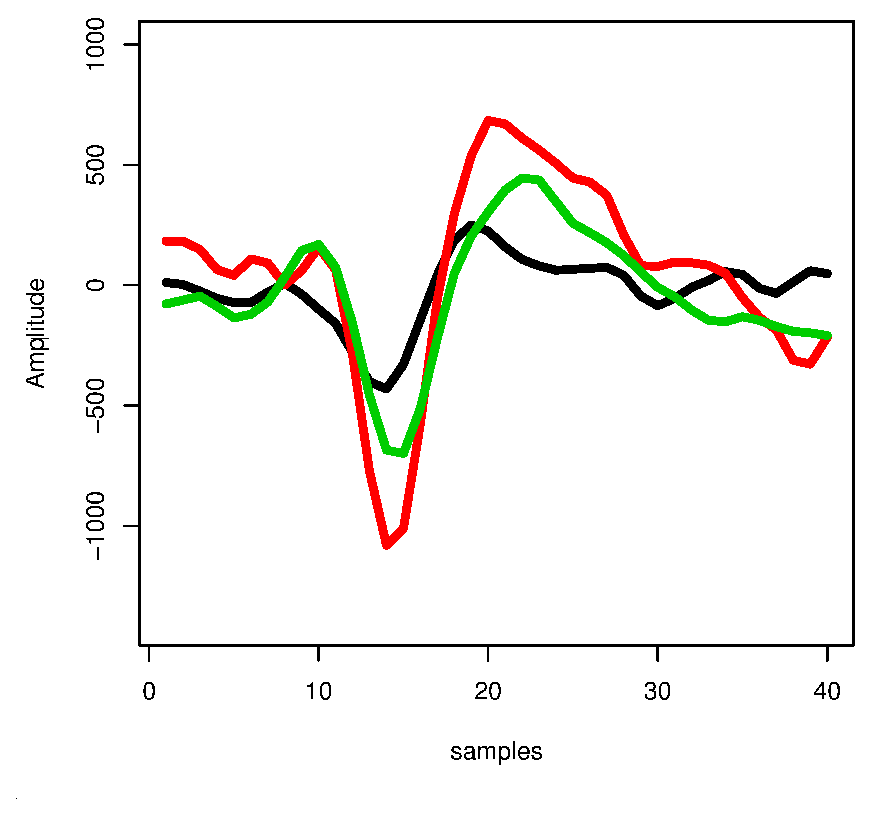
\includegraphics[width=15cm,keepaspectratio]{./fig/simu_1/template.eps}
	\caption{simulation 1: $B$=$l$>$l$N%F%s%W%l!<%HGH7A(B}
	\label{fig:simu_1_temps}
	\end{center}
\end{figure}

$B3F%9%Q%$%/GH7A$O!"<!$N(BEV$B%U%!%$%k$NCf$+$i!"GH7A$rFI$_9~$s$@$b$N$G$"$k!#(B
\begin{itemize}
 \item $B9u(B:04-9A\_ep013.005.ev
 \item $B@V(B:03-35Bep008.004.ev
 \item $BNP(B:0310d\_ep031.003.ev 
\end{itemize}
\clearpage
%\begin{figure}[htbp]
% \begin{tabular}{cc} %
%  \begin{minipage}{0.5\hsize}
%   \begin{center}
%    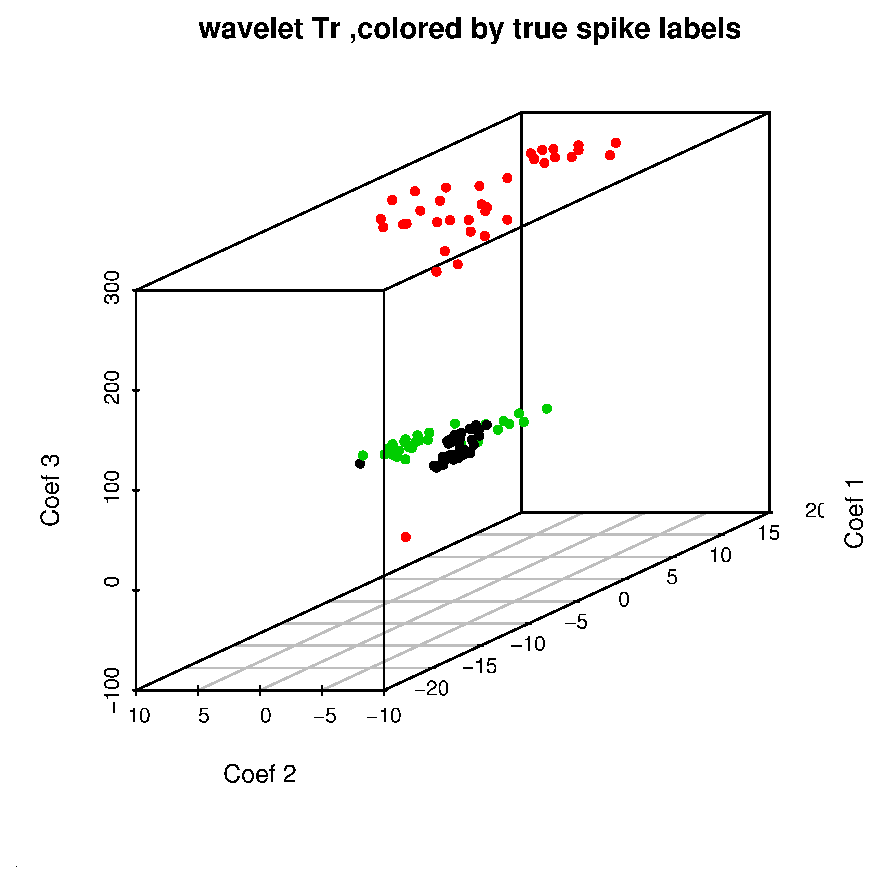
\includegraphics[width=9cm]{./fig/simu_1/SNR1wavelet_trueans.eps}
%  %  \caption{[A]}
%%    \label{fig_simu_1_trueans}  
%   \end{center}
%   \caption{simu1: true labels}
%   \label{fig_simu_1_trueans} 
%  \end{minipage}
%  
%  %k-means
%  \begin{minipage}{0.5\hsize}
%   \begin{center}
%    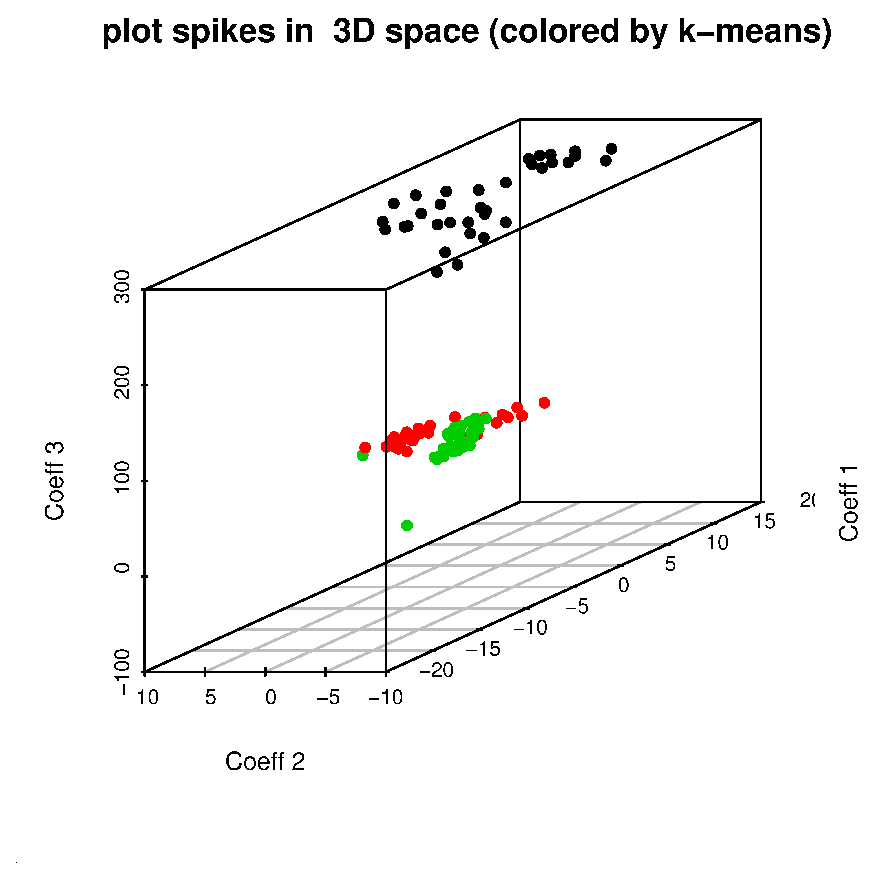
\includegraphics[width=9cm]{./fig/simu_1/SNR1wavelet_kmeans10.eps}
%    \caption{simu1: true labels}
%  \label{fig_simu_1_k-means} 
%   \end{center}
%  \end{minipage}
% \end{tabular}
% %\caption{[A]$B@5$7$$%9%Q%$%/%i%Y%k$H(B[B]$B%=!<%F%#%s%08e$N%9%Q%$%/%i%Y%k(B}
%% \label{fig_simu_1}
%\end{figure}
%
%%Wavelet Scores
%\begin{figure}
% \begin{center}
%    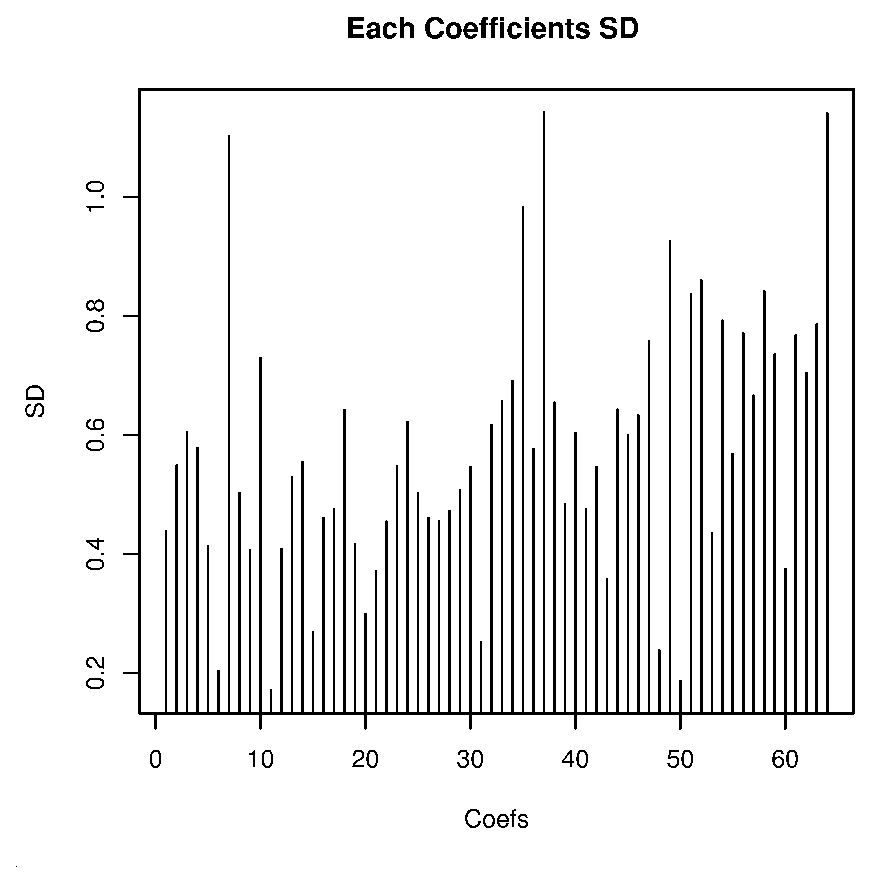
\includegraphics[width=10cm]{./fig/simu_1/SNR1Axes_Scores.eps}
% \end{center}
% \caption{Score}
% \label{simu_1_score}
%\end{figure}
%
%\clearpage


$B%7%_%e%l!<%7%g%s!!(B1
\begin{figure} [h] 
 \centering
 \hbox{
 %true

 \subfigure[$B@5$7$$%i%Y%k(B]{
 \label{fig_a} 
 \resizebox{8cm}{8cm}{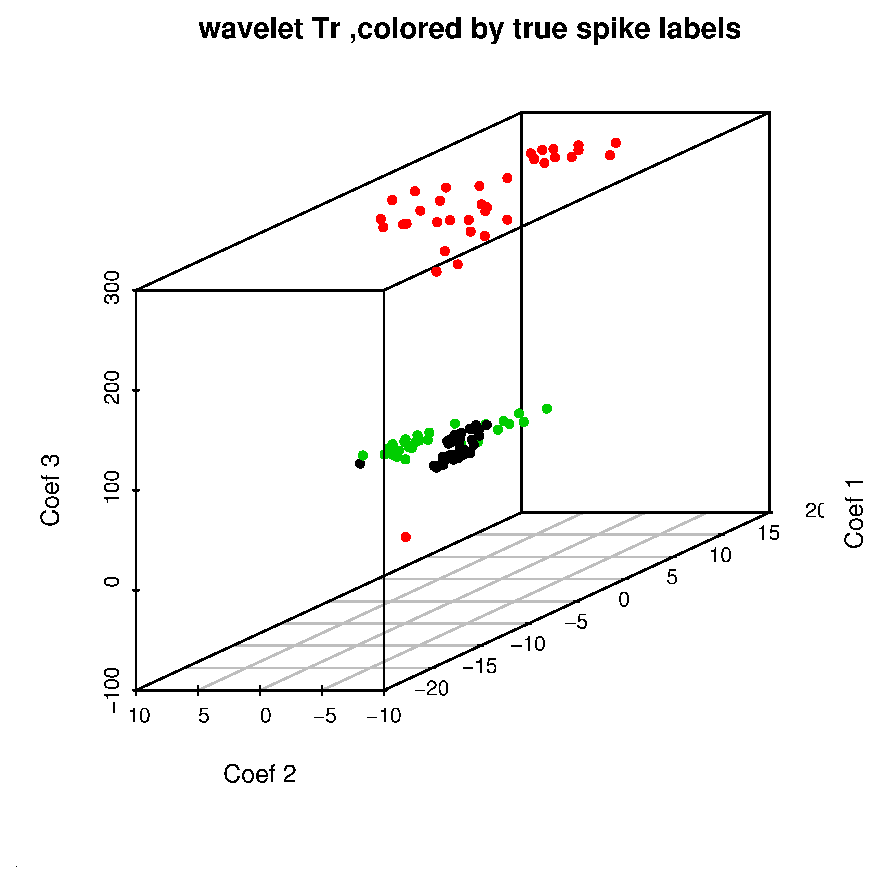
\includegraphics{./fig/simu_1/SNR1wavelet_trueans.eps}}}
 %k-means
 \subfigure[$B%=!<%F%#%s%08e(B]{
 \label{fig_b} 
 %\scalebox{0.3}{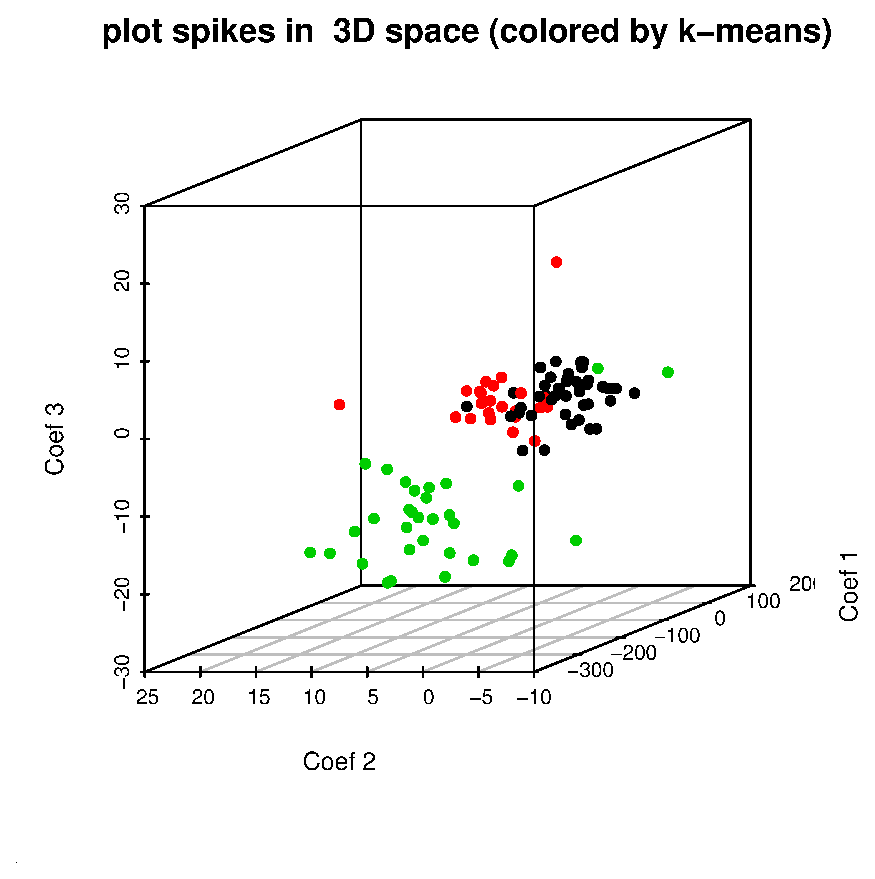
\includegraphics{./fig/simu_2/SNR1wavelet_kmeans10.eps}}}
 \resizebox{8cm}{8cm}{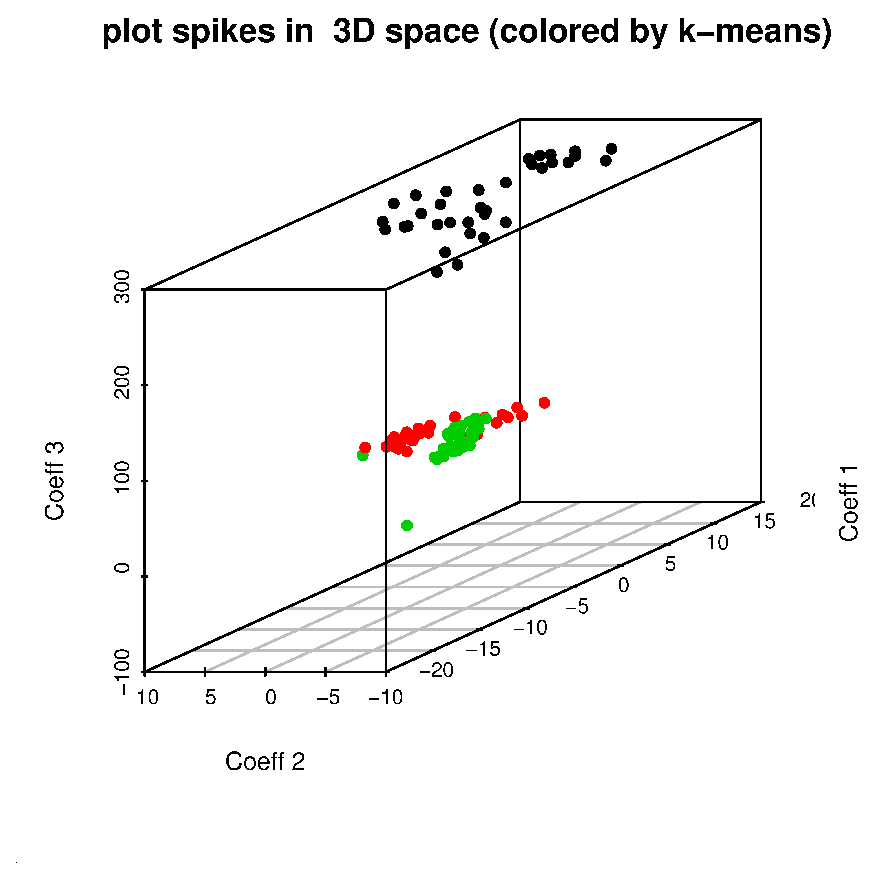
\includegraphics{./fig/simu_1/SNR1wavelet_kmeans10.eps}}}
}
\caption{simulation 1: $B%&%'!<%V%l%C%HJQ49$5$l$?%9%Q%$%/Ns(B}
%wavelet sd
%\subfigure[fig.c title]{
% \label{fig_c}
% \resizebox{10cm}{10cm}{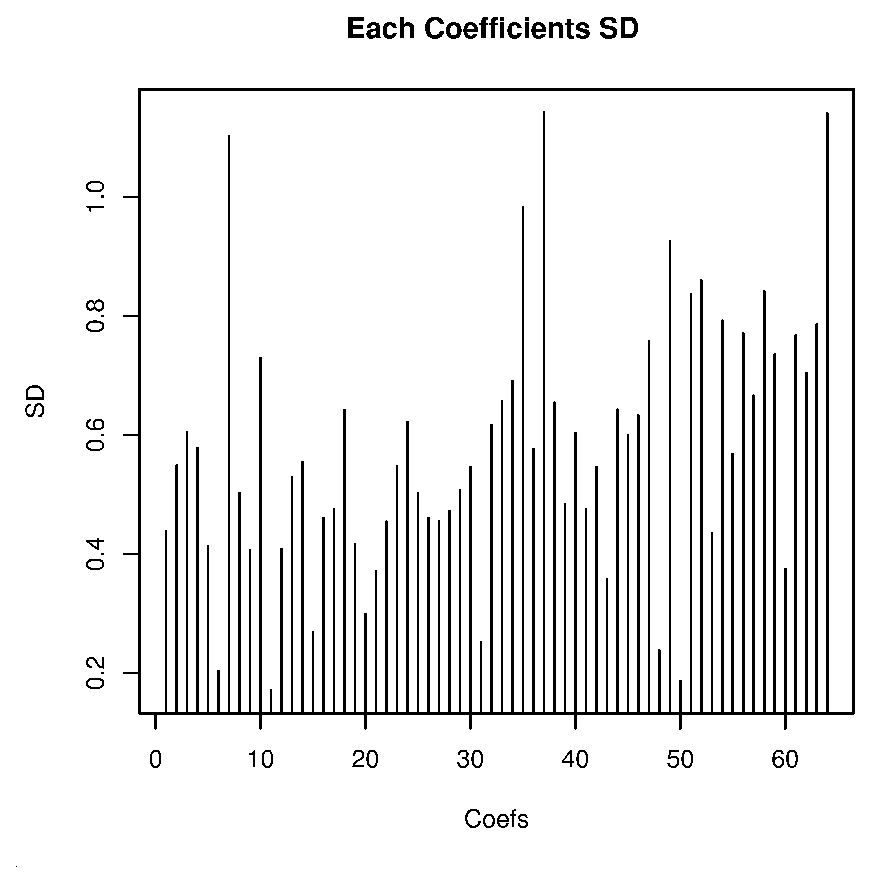
\includegraphics{./fig/simu_1/SNR1Axes_Scores.eps}}}
% \caption{$B4pDl4X?t(B$\phi_{1}\sim\phi_{64}$$B$NF@E@(B}
% \label{fig_total}
 \label{fig:simu_1}
\end{figure}

\begin{figure}[h]
 \begin{center}
    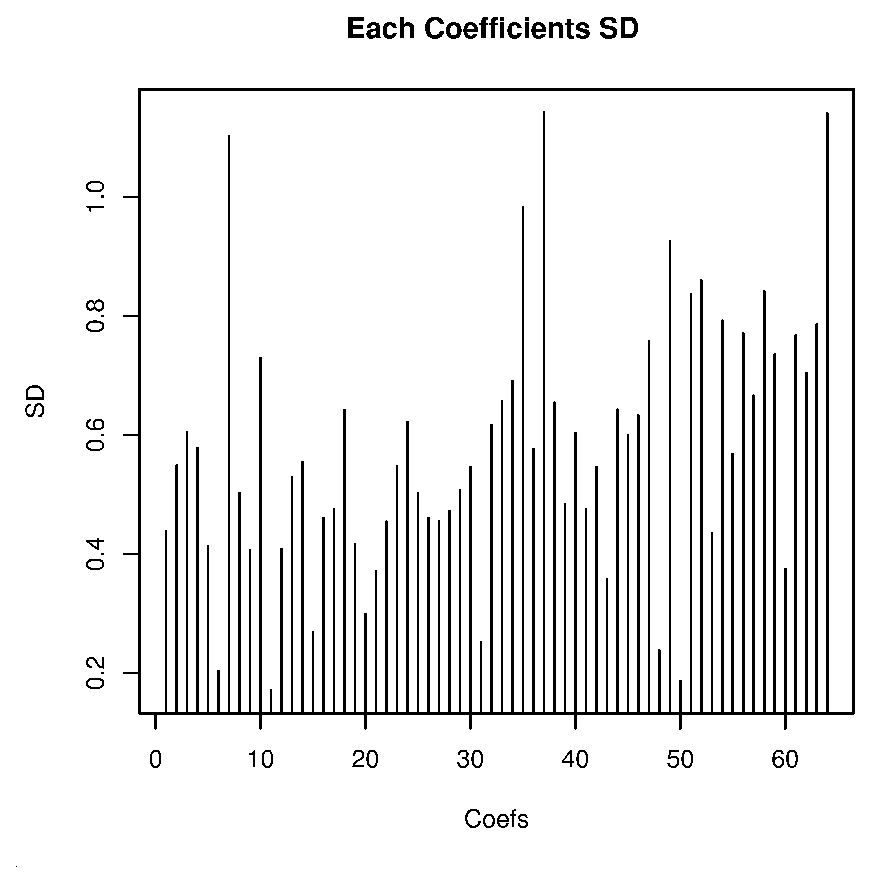
\includegraphics[width=7cm,height=7cm]{./fig/simu_1/SNR1Axes_Scores.eps}
 \end{center}
 \caption{simulation 1: $B4pDl4X?t(B$\phi_{1}\sim\phi_{64}$$B$NF@E@(B}
 \label{fig:simu_1_score}
\end{figure}


\clearpage